%
\newpage
\onecolumn
% \begin{minipage*}[\linewidth]{width of the minipage}
\renewcommand{\thesection}{\alph{section}}
\glsresetall
\setcounter{section}{0}

\section{Other \gls{cnn} models.}~\label{app:sec:other:models}
Variations in optimal threshold exist across models (Fig.~\ref{fig:sdm-appendix-a}). Like in Fig.~\ref{fig:detcurves}, the \gls{det} curves for three \gls{cnn}-based models, each trained on VGG2 with softmax but with different backbones.\footnote{Used pre-trained models and public Github, \href{https://github.com/rcmalli/keras-vggface}{https://github.com/rcmalli/keras-vggface}} Notice similar trends across subgroups and models, which is consistent with  Sphereface as well (Fig.~\ref{fig:detcurves}). For example, the plots generated with Spherface and VggFace2 all have the \gls{wm} curve at the bottom (\ie best) and \gls{af} on top (\ie worst). 
% ArcFace (not shown) shown similar results. We would have to cite + will incorporate later .... a blank statement and sphereface is comparable ... up to you i do not care
% \begin{figure}[h!]
% % \vspace{-2mm}
%     \centering
%     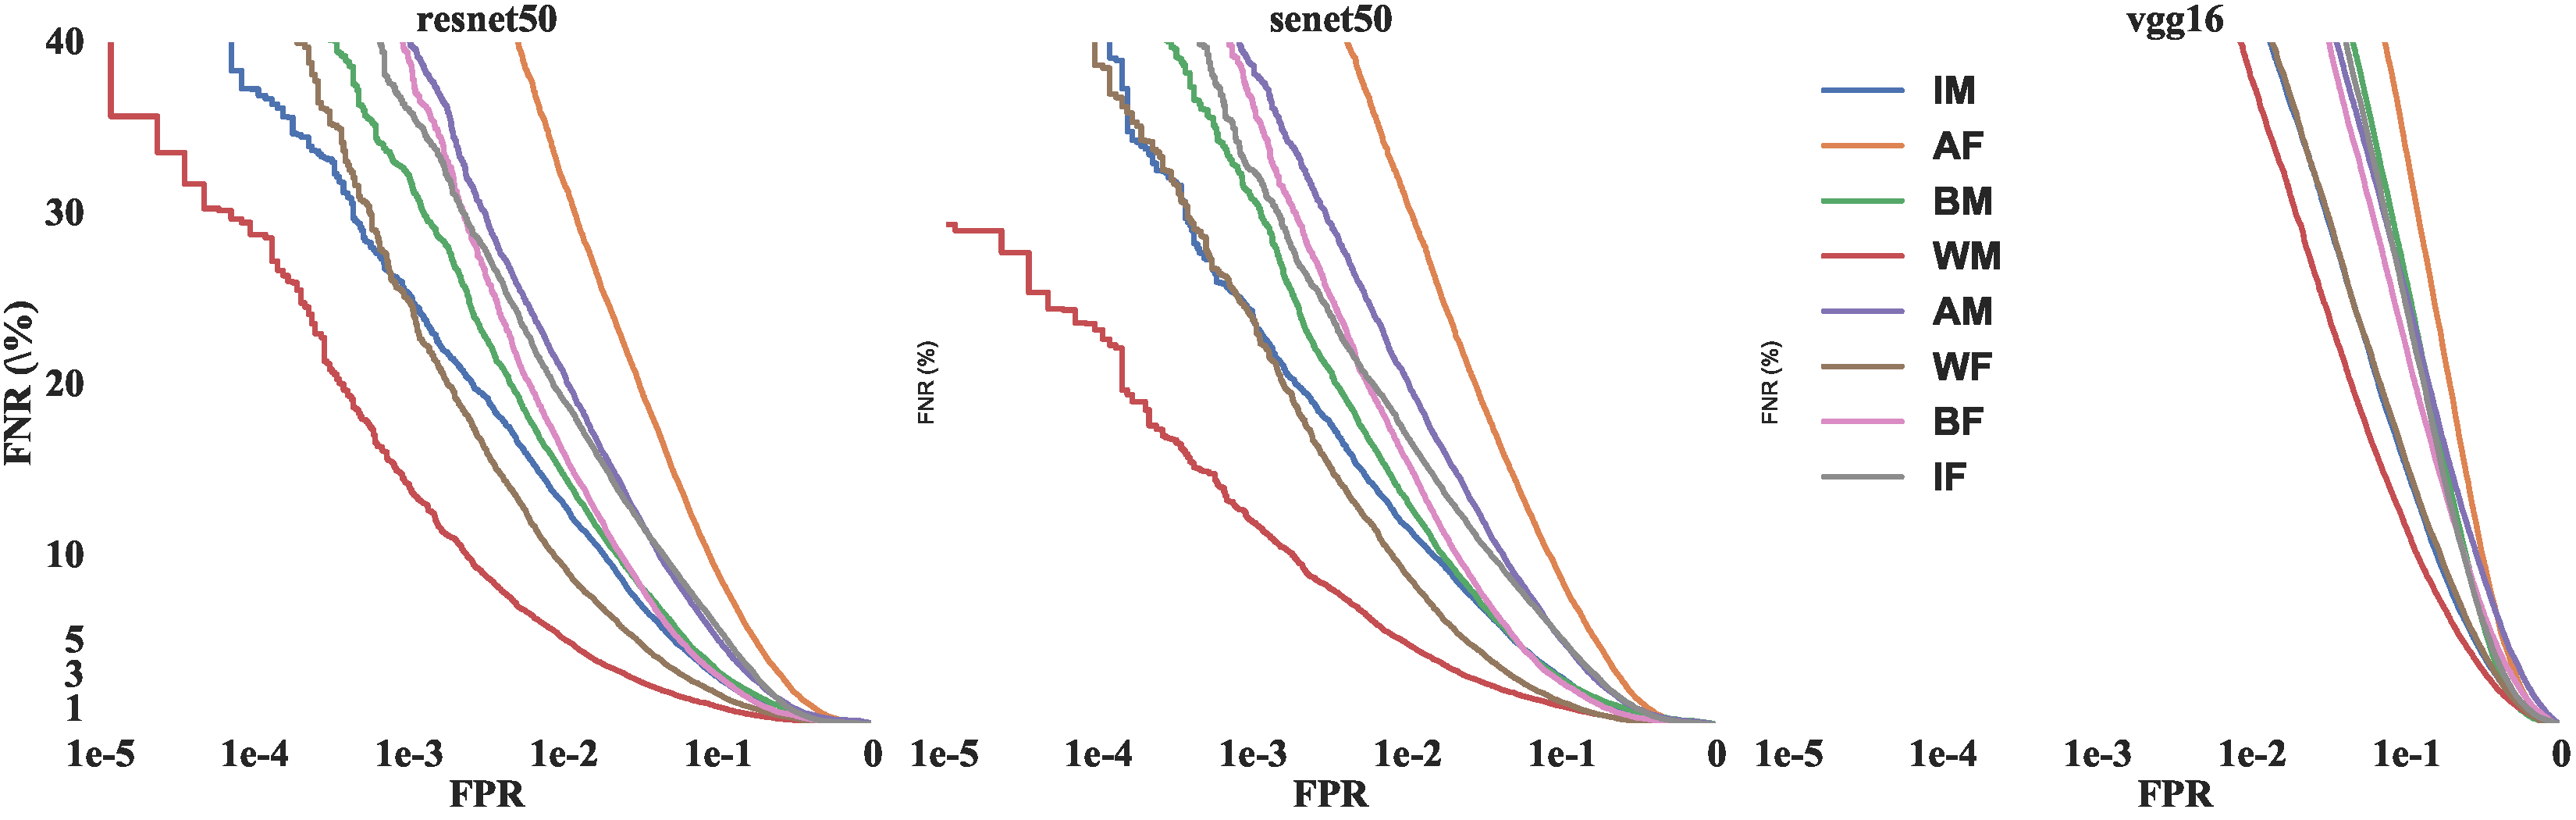
\includegraphics[width=.8\linewidth, trim={0mm 0mm 0mm 0mm},clip]{figures/SDM.pdf}\\
%     \caption{\textbf{\gls{det} curves for different CNN models}. \gls{fnr} (\%) (vertical) vs \gls{fpr} (log-scale)  (horizontal) for VGG2~\cite{Cao18} models with different backbones (vgg16, Resnet50~\cite{he2016deep}, SEnet50~\cite{hu2018squeeze}). Lower is better. For each plot, \gls{wm} is the best performing curve, \gls{af} is the worst. The the ordering of the curves is roughly the same for each backbone.}\label{fig:sdm-appendix-a}
%     \vspace{-3mm}
% \end{figure}


\begin{figure}[h!]
\vspace{-1mm}
    \centering
    \begin{subfigure}[t]{.3\linewidth}
    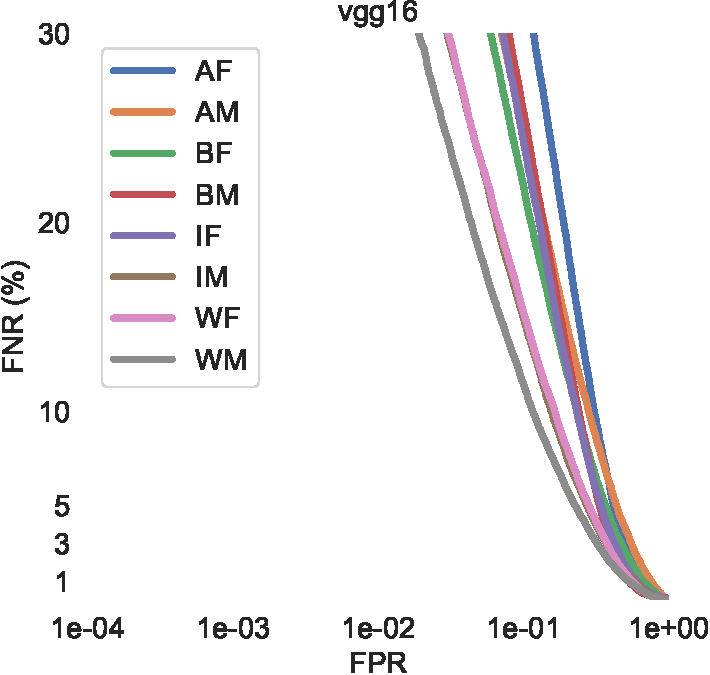
\includegraphics[width=.75\linewidth]{figures/curve_vgg16_subgroups-crop.pdf}
    \caption{VGG16~\cite{simonyan2014very}}
 \end{subfigure}
    \begin{subfigure}[t]{.27\linewidth}
    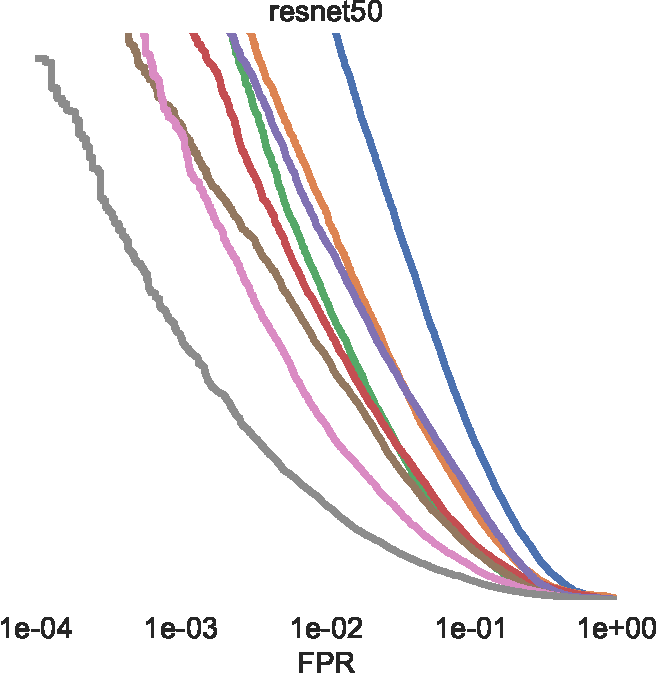
\includegraphics[width=.8\linewidth]{figures/curve_resnet50_subgroups-crop.pdf}
    \caption{ResNet50~\cite{he2016deep}}
   \end{subfigure}
    \begin{subfigure}[t]{.27\linewidth}
    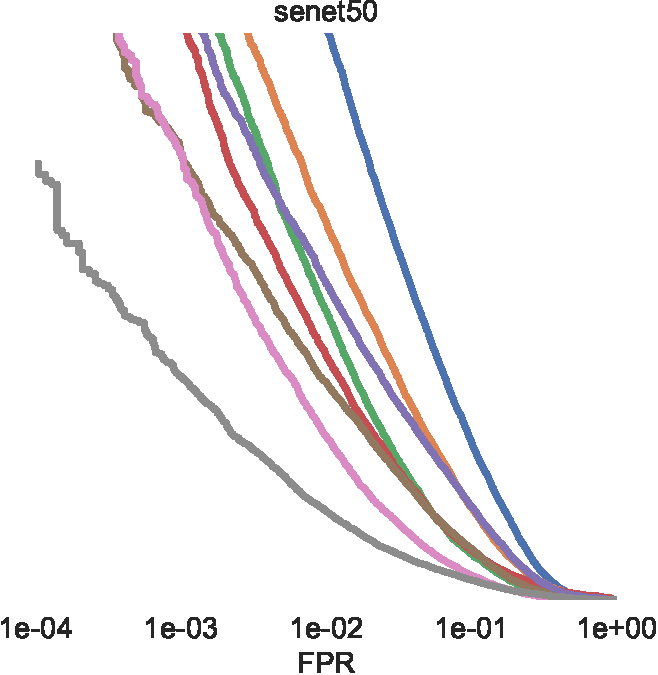
\includegraphics[width=.8\linewidth]{figures/curve_senet50_subgroups-crop.pdf}
    \caption{SENet~\cite{hu2018squeeze}}
    \end{subfigure}
    \caption{\textbf{\gls{det} curves for different CNN models}. \gls{fnr} (\%) (vertical) vs \gls{fpr} (log-scale)  (horizontal) for VGG2~\cite{Cao18} models with different backbones (VGG16, Resnet50, SEnet50). Lower is better. For each plot, \gls{wm} is the best performing curve, \gls{af} is the worst. The the ordering of the curves is roughly the same for each backbone.}\label{fig:sdm-appendix-a}
    \vspace{-1mm}
\end{figure}



Sample faces per subgroup of the \gls{bfw} dataset are shown in Fig.~\ref{fig:montage:app}.
\begin{figure}[h!]
\vspace{-2mm}
    \centering
    \includegraphics[width=.7\linewidth]{figures/facemontage.pdf}
    \caption{\textbf{Sample of \gls{bfw}}. Each row depicts a different gender, \gls{f} (top) and \gls{m} (bottom). Columns are grouped by ethnicity (\ie \gls{a}, \gls{b}, \gls{i}, and \gls{w}, respectfully).}
    \label{fig:montage:app}
    \vspace{-1mm}
\end{figure}
{
\scriptsize
\begin{thebibliography}{widest entry}
 \bibitem[1]{Cao18} Qiong Cao, Li Shen, Weidi Xie, Omkar M. Parkhi, and Andrew Zisserman. ``Vggface2: A dataset for recognising faces across pose and age.'' In \textit{IEEE International Conference on Automatic Face \& Gesture Recognition.} 2018.
 \bibitem[2]{simonyan2014very} Karen Simonyan and Andrew Zisserman. ``Very deep convolutional networks for large-scale image recognition'' \textit{arXiv preprint arXiv:1409.1556.} 2014.
  \bibitem[3]{he2016deep} He, Kaiming, Xiangyu Zhang, Shaoqing Ren, and Jian Sun. ``Deep residual learning for image recognition.'' In \textit{IEEE Conference on Computer Vision and Pattern Recognition.} 2016.
 \bibitem[4]{hu2018squeeze} Hu, Jie, Li Shen, and Gang Sun. ``Squeeze-and-excitation networks.'' In \textit{IEEE Conference on Computer Vision and Pattern Recognition.} 2018.
\end{thebibliography}
}

% \end{minipage*}